%%%%%%%%%%%%%%%%%%%%%%%%%%%%%%%%%%%%%%%%%
% Journal Article
% LaTeX Template
% Version 1.3 (9/9/13)
%
% This template has been downloaded from:
% http://www.LaTeXTemplates.com
% http://en.wikibooks.org/wiki/LaTeX/Mathematics
% Original author:
% Frits Wenneker (http://www.howtotex.com)
%
% License:
% CC BY-NC-SA 3.0 (http://creativecommons.org/licenses/by-nc-sa/3.0/)
%
%%%%%%%%%%%%%%%%%%%%%%%%%%%%%%%%%%%%%%%%%

%----------------------------------------------------------------------------------------
%	PACKAGES AND OTHER DOCUMENT CONFIGURATIONS
%----------------------------------------------------------------------------------------

%\documentclass[twoside]{article}
\documentclass[a4paper,12pt]{article}

%\usepackage{lipsum} % Package to generate dummy text throughout this template
\usepackage{mathtools} % package fixes some amsmath quirks and adds some useful settings, symbols, and environments to amsmath
\usepackage[sc]{mathpazo} % Use the Palatino font
\usepackage[T1]{fontenc} % Use 8-bit encoding that has 256 glyphs
\linespread{1.05} % Line spacing - Palatino needs more space between lines
\usepackage{microtype} % Slightly tweak font spacing for aesthetics

\usepackage[hmarginratio=1:1,top=32mm,columnsep=20pt]{geometry} % Document margins
\usepackage{multicol} % Used for the two-column layout of the document
\usepackage[hang, small,labelfont=bf,up,textfont=it,up]{caption} % Custom captions under/above floats in tables or figures
\usepackage{booktabs} % Horizontal rules in tables
\usepackage{float} % Required for tables and figures in the multi-column environment - they need to be placed in specific locations with the [H] (e.g. \begin{table}[H])
\usepackage{hyperref} % For hyperlinks in the PDF

\usepackage{lettrine} % The lettrine is the first enlarged letter at the beginning of the text
\usepackage{paralist} % Used for the compactitem environment which makes bullet points with less space between them

\usepackage{cite}
%\usepackage[numbers,sort&compress]{natbib}
%\usepackage[style=numeric]{biblatex}
%\addbibresource{thomastsai.bib}
%\bibliographystyle{ieeetr}

\usepackage{abstract} % Allows abstract customization
\renewcommand{\abstractnamefont}{\normalfont\bfseries} % Set the "Abstract" text to bold
\renewcommand{\abstracttextfont}{\normalfont\small\itshape} % Set the abstract itself to small italic text

%http://en.wikibooks.org/wiki/LaTeX/Floats,_Figures_and_Captions
\usepackage{graphicx}
\usepackage{subcaption}
\graphicspath{ {dft/} }
\DeclareGraphicsExtensions{.pdf,.png,.jpg}

\usepackage{titlesec} % Allows customization of titles
\renewcommand\thesection{\Roman{section}} % Roman numerals for the sections
\renewcommand\thesubsection{\Roman{subsection}} % Roman numerals for subsections
\titleformat{\section}[block]{\large\scshape\centering}{\thesection.}{1em}{} % Change the look of the section titles
\titleformat{\subsection}[block]{\large}{\thesubsection.}{1em}{} % Change the look of the section titles

\usepackage{fancyhdr} % Headers and footers
\pagestyle{fancy} % All pages have headers and footers
\fancyhead{} % Blank out the default header
\fancyfoot{} % Blank out the default footer
\fancyhead[C]{DSP Study $\bullet$ 2015 $\bullet$ Vol. XXI, No. 1} % Custom header text
%\fancyfoot[RO,LE]{\thepage} % Custom footer text
\fancyfoot[RO,L]{\thepage} % Custom footer text

%----------------------------------------------------------------------------------------
%	TITLE SECTION
%----------------------------------------------------------------------------------------

\title{\vspace{-15mm}\fontsize{24pt}{10pt}\selectfont\textbf{DSP Study}} % Article title

\author{
\large
\textsc{Thomas Tsai}\thanks{VP of BioTrump RD}\\[2mm] % Your name
\normalsize www.biotrump.com \\ % Your institution
\normalsize \href{mailto:thomas@biotrump.com}{thomas@biotrump.com} % Your email address
\vspace{-5mm}
}
\date{}

%----------------------------------------------------------------------------------------

\begin{document}

\maketitle % Insert title

\thispagestyle{fancy} % All pages have headers and footers

%----------------------------------------------------------------------------------------
%	ABSTRACT
%----------------------------------------------------------------------------------------

\begin{abstract}

%\noindent \lipsum[1] % Dummy abstract text
Independent component analysis, ICA, needs whitening the input signals.

\end{abstract}

%----------------------------------------------------------------------------------------
%	ARTICLE CONTENTS
%----------------------------------------------------------------------------------------

%\begin{multicols}{2} % Two-column layout throughout the main article text
%\end{multicols}
%\onecolumn

\section{Introduction}

\lettrine[nindent=0em,lines=3]{R}\ ADICAL Independent Component Analysis, \textbf{RADICAL ICA},
\cite{radical-ica} \cite{journals/informaticaSI/NaikK11} are used for pulse rate analysis.
RADICAL is the best method to solve ICA problems.
%\lipsum[2-3] % Dummy text

%------------------------------------------------

\section{axioms}

\begin{compactitem}
\item If A is a n*n square matrix. Eigen value $\lambda$ and \textbf{eigen} vector $\hat{x}$: \cite{AntonELA10th}
\begin{equation}
\label{eq:eval}
A\hat{x}=\lambda \hat{x}
\end{equation}
The sign of $\lambda$ and $\hat{x}$ are not unique. And $\lambda$ and $\hat{x}$ are scalable.

\item A symmetric square matrix, $A=A^T$, can be eigen decomposition which is a special form of
singular value decomposition, SVD, of a m*n matrix.
\begin{equation}
\label{eq:PDP}
A = PDP^{T}\ or\ U \Lambda U^T\
\end{equation}
where \textbf{D or $\Lambda$} is a \textbf{diagonal matrix} whose diagonal components are eigen values.\\

\begin{equation}
\label{eq:diagm}
D=\Lambda= diag(\lambda_{ii}) = \begin{pmatrix}
       \lambda_{00}& 0 				& ..	&	0 	\\[0.3em]
       0 			& \lambda_{11} & ..		&	0 	\\[0.3em]
       .			& .				& ..	&	.	\\[0.3em]
       0 			& 0 			& ..	&	\lambda_{nn}\\[0.3em]
     \end{pmatrix}
\end{equation}

P or U is composed of orthonormal eigen vectors, so $P^{-1}=P^T$ or $U^{-1}=U^T$.\\
P or U is invertable and nonsigular. $det(P) \neq0$
\begin{equation}
\label{eq:pdpI}
I=P* P^{-1} = P* P^T=U* U^{-1} = U* U^T
\end{equation}

This decomposition \eqref{eq:PDP} is not unique, because $\Lambda$ and $U$ are not unique.
When the diagonal elements, eigen value, of the diagonal matrix, $\Lambda$, are changed in the order.
$U$ is also changed .

\item The diagonal matrix properties:\\
The determinant of D is the product of all the diagonal elements.
\begin{equation}
\label{eq:detD}
det(D) = \prod_{i}^{} \lambda_{ii}
\end{equation}\\

\begin{equation}
\label{eq:pdpD}
D^{-1}=\Lambda^{-1}=diag(\lambda_{ii}^{-1})=
\begin{pmatrix}
       1/\lambda_{00}& 0 				& ..	&	0 	\\[0.3em]
       0 			& 1/\lambda_{11} & ..		&	0 	\\[0.3em]
       .			& .				& ..	&	.	\\[0.3em]
       0 			& 0 			& ..	&	1/\lambda_{nn}\\[0.3em]
\end{pmatrix}
\end{equation}\\
\begin{equation}
\label{eq:det-pdpD}
\\
det(D^{-1})=det(\Lambda^{-1})=
\prod_{i}^{} \frac{1}{\lambda_{ii} }\\
=\prod_{i}^{} \lambda_{ii}^{-1} \\
\end{equation}\\

\item standard deviation and variance:
\begin{equation}
\label{eq:std}
\sigma = \sqrt {\sum \frac{(x-\bar{x})^2}{N}}
\end{equation}
\begin{equation}
\label{eq:variance}
VAR(X)=\sigma^{2} = {\sum \frac{(x-\bar{x})^2}{N}}
\end{equation}

\item covariance: X and Y are two vectors, random variables. The covariance is a value.
\begin{equation}
\label{eq:covar}
Cov(X,Y)=\sigma(X,Y)=E[(X - E[X])(Y-E[Y])]
\end{equation}
\begin{equation}
\label{eq:covar1}
Cov(X,Y)=\frac{\sum(X_i-\bar{X})(Y_i-\bar{Y})}{N}=
\frac{\sum(x_i)(y_i)}{N}
\end{equation}
Deviation score $x_i, y_i$:
\begin{equation}
\label{eq:covar1}
x_{i}=(X_i-\bar{X}),\;
y_{i}=(Y_i-\bar{Y})
\end{equation}
Variance of X, $VAR(X)=Cov(X,X)=\sigma^{2}$, \ is a degenerated form of covariance.\\

\item covariance matrix: is a measure of the extent to which corresponding elements from two sets
of ordered data move in the same direction. We use the following formula to compute covariance.
\cite{wiki-covariance}\cite{STAT-covariance}\\
\\Let $X_i$ be the \textbf{column} vector in a Matrix \textbf{X}=
$\begin{pmatrix} X_1 & X_2 &... & X_c \end{pmatrix}$\\
The covariance matrix of \textbf{X} is:\\
$M_{cxc} = \Sigma{(\textbf{X})}=$
\[
\begin{pmatrix}
       COV(X_1,X_1) 	& COV(X_1,X_2) 	& ...	& COV(X_1,X_c)	\\[0.3em]
       COV(X_2,X_1) 	& COV(X_2,X_2) 	& ...	& COV(X_2,X_c)	\\[0.3em]
       ...		& ...			& ...	&	...		\\[0.3em]
       COV(X_c,X_1) 	& COV(X_c,X_2) 	& ...	& COV(X_c,X_c)	\\[0.3em]
\end{pmatrix}
=\]
\begin{equation}
\label{eq:covarm1}
\begin{pmatrix}
       \sum x_{1i}^{2}/N 	& \sum x_{1i} x_{2i}/N 	& ...	& \sum x_{1i} x_{ci}/N	\\[0.3em]
       \sum x_{2i} x_{1i}/N 	& \sum x_{2i} x_{2i}/N 	& ...	& \sum x_{2i} x_{ci}/N	\\[0.3em]
       ...		& ...			& ...	&	...		\\[0.3em]
       \sum x_{ci} x_{1i}/N 	& \sum x_{ci} x_{2i}/N 	& ...	& \sum x_{ci}^{2}/N	\\[0.3em]
\end{pmatrix}
=(1/N)
\begin{pmatrix}
       \sum x_{1i}^{2} 	& \sum x_{1i} x_{2i} 	& ...	& \sum x_{1i} x_{ci}	\\[0.3em]
       \sum x_{2i} x_{1i} 	& \sum x_{2i} x_{2i} 	& ...	& \sum x_{2i} x_{ci}	\\[0.3em]
       ...		& ...			& ...	&	...		\\[0.3em]
       \sum x_{ci} x_{1i} 	& \sum x_{ci} x_{2i} 	& ...	& \sum x_{ci}^{2}	\\[0.3em]
\end{pmatrix}
\end{equation}
where\\
N is the dim of the column vector $X_i$.\\
$x_i$ is a deviation score from the ith data set.\\
$\sum x_i^2 / N$ is the variance of elements from the ith data set.\\
$\sum x_i x_j / N$ is the covariance for elements from the ith and jth data sets.\\

\item Properties of Covariance matrix : $\Sigma(\textbf{X})$ \\
\textbf{square and symmetric}: $M_{cxc}=M_{cxc}^T$ ,\ because $\sum x_i x_j / N$ and $\sum x_j x_i / N$ are the same. Refer to \eqref{eq:PDP}
\begin{equation}
\label{eq:covd}
\Sigma(\textbf{X}) = U\Lambda U^T
\end{equation}

\textbf{linearity of expectation matrix}: Let \textbf{X} be a random vector with covariance matrix
$\Sigma(\textbf{X})$, and let A be a matrix that can act on \textbf{X}. The covariance matrix of the vector A\textbf{X} is:
\begin{equation}
\label{eq:covlinear}
\Sigma(A\textbf{X}) = A\Sigma(\textbf{X})A^{T}
\end{equation}

\item whiten: Refer to \eqref{eq:covd},  A \textbf{whitening} matrix W is defined as
\begin{equation}
\label{eq:whitem}
W=\Lambda^{-1/2} U^{T}
\end{equation}
This W is not unique, because $\Lambda$ and $U^T$ are not unique.
When the diagonal elements, eigen value, of the diagonal matrix, $\Lambda$, are changed in the order.
$U$ is also changed .

Let
\begin{equation}
\label{eq:whitened}
Y = W*\textbf{X}= (\Lambda^{-1/2} U^{T}) \textbf{X}
\end{equation}
be a \textbf{whitened matrix} of \textbf{X}.\\
The covariance matrix of Y which is a whitened matrix of X.
\[
\Sigma (Y)=\Sigma (\Lambda^{-1/2} U^{T}) \textbf{X}
\]
Refer to the equation \eqref{eq:covlinear}
\[
A=(\Lambda^{-1/2} U^{T})
\]
so
\[
\Sigma (Y)=\Sigma (\Lambda^{-1/2} U^{T}) \textbf{X}=
(\Lambda^{-1/2} U^{T})(\Sigma (\textbf{X})) (\Lambda^{-1/2} U^{T})^{T}
\]
Refer to the equation \eqref{eq:covd}\\
$=(\Lambda^{-1/2} U^{T}) (U \Lambda U^{T}) (\Lambda^{-1/2} U^{T}) ^T$\\
$=\Lambda^{-1/2} (U^{T}  U) \Lambda U^{T} (\Lambda^{-1/2} U^{T}) ^T$\\
Refer to the equation \eqref{eq:pdpI}\\
$=\Lambda^{-1/2} (I) \Lambda U^{T} ({U^{T}}^T{\Lambda^{-1/2}}^T)$\\
$=\Lambda^{-1/2} \Lambda U^{T} (U{\Lambda^{-1/2}}^T)$\\
$=\Lambda^{-1/2} \Lambda (U^{T} U) {\Lambda^{-1/2}}^T$\\
$=\Lambda^{-1/2} \Lambda (I) {\Lambda^{-1/2}}^T$\\
$=\Lambda^{-1/2} \Lambda \Lambda^{-1/2}$\\
$=\Lambda^{(-1/2) + (1) + (-1/2)}$\\
$=I$\\
So \textbf{Y is whitened}, because it's covariance matrix is a Identity matrix.
All column vectors in Y has no correlation!

\item \textbf{Simplification} for a \textbf{normalized} vector $\hat{X_i}$:\\
Let \textbf{X}=$\begin{pmatrix} X_1 & X_2 & ... & X_c \end{pmatrix}, X_1,X_2,X_c$ are column vectors which have been normalized.
(zero mean and unit variance)\\

Refer to the equation \eqref{eq:covar1}, Deviation score $x_k, y_k$:\\
$x_{k}=(X_{ik}-\bar{X_i})=(X_{ik} - 0)= X_{ik}$ \\
$y_{k}=(Y_{ik}-\bar{Y_i})=(Y_{ik} - 0) = Y_{ik}$


Refer to the equation \eqref{eq:covarm1}, covariance matrix $\Sigma(\textbf{X})$=
\[
(1/N)
\begin{pmatrix}
       \sum x_{1k}^{2} 	& \sum x_{1k} x_{2k} 	& ...	& \sum x_{1k} x_{ck}	\\[0.3em]
       \sum x_{2k} x_{1k} 	& \sum x_{2k} x_{2k} 	& ...	& \sum x_{2k} x_{ck}	\\[0.3em]
       ...		& ...			& ...	&	...		\\[0.3em]
       \sum x_{ck} x_{1k} 	& \sum x_{ck} x_{2k} 	& ...	& \sum x_{ck}^{2}	\\[0.3em]
\end{pmatrix}
\]
\[
=(1/N)
\begin{pmatrix}
       \sum X_{1k}^{2} 	& \sum X_{1k} X_{2k} 	& ...	& \sum X_{1k} X_{ck}	\\[0.3em]
       \sum X_{2k} X_{1k} 	& \sum X_{2k} X_{2k} 	& ...	& \sum X_{2k} X_{ck}	\\[0.3em]
       ...		& ...			& ...	&	...		\\[0.3em]
       \sum X_{ck} X_{1k} 	& \sum X_{ck} X_{2k} 	& ...	& \sum X_{ck}^{2}	\\[0.3em]
\end{pmatrix}
\]
\[
=(1/N)
\begin{pmatrix}
       \langle X_1, X_1 \rangle	& \langle X_1, X_2 \rangle 	& ...	& \langle X_1, X_c	\rangle \\[0.3em]
       \langle X_2, X_1 \rangle 	& \langle X_2, X_2 \rangle	& ...	& \langle X_2, X_c	\rangle \\[0.3em]
       ...		& ...			& ...	&	...		\\[0.3em]
       \langle X_c, X_1 \rangle	& \langle X_c, X_2 \rangle 	& ...	& \langle X_c, X_c\rangle	\\[0.3em]
\end{pmatrix}
\]
Let \textbf{X}=$\begin{pmatrix} R & G & B \end{pmatrix}$, R,G,B are column vectors which have been normalized.
\[
R=
\begin{pmatrix}
       R_0\\[0.3em]
       R_1\\[0.3em]
       R_2\\[0.3em]
       R_3\\[0.3em]
		. \\[0.3em]
       R_{n-1}\\[0.3em]
\end{pmatrix}
, G=
\begin{pmatrix}
       G_0\\[0.3em]
       G_1\\[0.3em]
       G_2\\[0.3em]
       G_3\\[0.3em]
		. \\[0.3em]
       G_{n-1}\\[0.3em]
\end{pmatrix}
, B=
\begin{pmatrix}
       B_0\\[0.3em]
       B_1\\[0.3em]
       B_2\\[0.3em]
       B_3\\[0.3em]
		. \\[0.3em]
       B_{n-1}\\[0.3em]
\end{pmatrix}
\]

\[
\Sigma(\textbf{X})=(1/N)
\begin{pmatrix}
       \langle R, R \rangle	& \langle R, G \rangle 	& \langle R, B	\rangle \\[0.3em]
       \langle G, R \rangle 	& \langle G, G \rangle		& \langle G, B	\rangle \\[0.3em]
       \langle B, R \rangle	& \langle B, G \rangle 	& \langle B, B	\rangle	\\[0.3em]
\end{pmatrix}
=
\begin{pmatrix}
       \sigma_R^2              & \langle R, G \rangle 	&  \langle R, B	\rangle \\[0.3em]
       \langle G, R \rangle 	& \sigma_G^2	            & \langle G, B	\rangle \\[0.3em]
       \langle B, R \rangle	& \langle B, G \rangle 	& \sigma_B^2	\\[0.3em]
\end{pmatrix}
\]
\[
=
\begin{pmatrix}
       R_0 & R_1 & R_2 & R_3 ... & R_{n-1} \\[0.3em]
       G_0 & G_1 & G_2 & G_3 ... & G_{n-1} \\[0.3em]
       B_0 & B_1 & B_2 & B_3 ... & B_{n-1} \\[0.3em]
\end{pmatrix}
\begin{pmatrix}
       R_0     & G_0     & B_0\\[0.3em]
       R_1     & G_1     & B_1\\[0.3em]
       R_2     & G_2     & B_2\\[0.3em]
       R_3     & G_3     & B_3\\[0.3em]
		.      & .       & .  \\[0.3em]
       R_{n-1} & G_{n-1} & B_{n-1}\\[0.3em]
\end{pmatrix}
=
\begin{pmatrix}
       R \\[0.3em]
       G \\[0.3em]
       B \\[0.3em]
\end{pmatrix}
\begin{pmatrix}
       R & G & B\\[0.3em]
\end{pmatrix}
\]
The time complexity is $O(N^2)$.\\
Because R,G,B are zero mean and unit variance, $\sigma^2=1$.
\begin{equation}
\label{eq:covar-norm-RGB}
\Sigma(\textbf{X})=(1/N)
\begin{pmatrix}
       1 							& \langle R, G \rangle 	& \langle R, B	\rangle \\[0.3em]
       \langle G, R \rangle 		& 1							& \langle G, B	\rangle \\[0.3em]
       \langle B, R \rangle		& \langle B,G  \rangle 	& 1	\\[0.3em]
\end{pmatrix}
= U\Lambda U^T
\end{equation}
The diagonal elements are all "1", and $\Sigma(\textbf{X})$ is a symmetric matrix, so only 3 items are computed: $\langle R, G \rangle$, $\langle R, B	\rangle$, $\langle G, B	\rangle$
\\The computing complexity can be reduced very much to be $O(\binom {N}{2})=O(C_2^N) = O(N^2/2)$.


\end{compactitem}

%\lipsum[4] % Dummy text

%------------------------------------------------

\section{Fourier Transform}

\subsection{Continuous Fourier Transform}

\subsection{Discrete Fourier Transform}
\begin{figure}[ht]
  \label{fig:F_10_9}
  \centering
	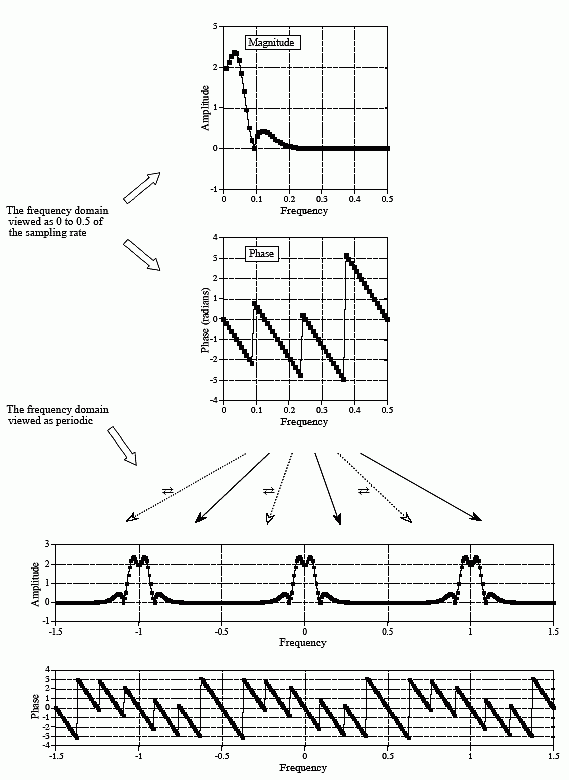
\includegraphics[width=0.7\textwidth, keepaspectratio=true]{F_10_9}
	\caption{.}
\end{figure}


\begin{figure}[h!]
 \label{fig:F_8_3}
 \centering
 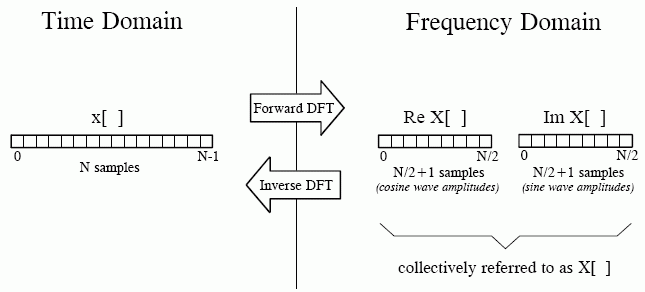
\includegraphics[width=\textwidth, keepaspectratio=true]{F_8_3}
 \caption{In the time domain, x[] consists of N points running from 0 to N-1. In the frequency domain,
the DFT produces two signals, the real part, written: ReX[], and the imaginary part, written: Im X[ ]. Each of
these frequency domain signals are N/2+1 points long, and run from 0 to N/2. The Forward DFT transforms from
the time domain to the frequency domain, while the Inverse DFT transforms from the frequency domain to the
time domain. (Take note: this figure describes the real DFT. The complex DFT, discussed in Chapter 31,
changes N complex points into another set of N complex points).}
\end{figure}
%\autoref{fig:F_8_3}

\subsection{Fast Fourier Transform}

\begin{figure}
  \label{fig:F_12_1}
  \centering
	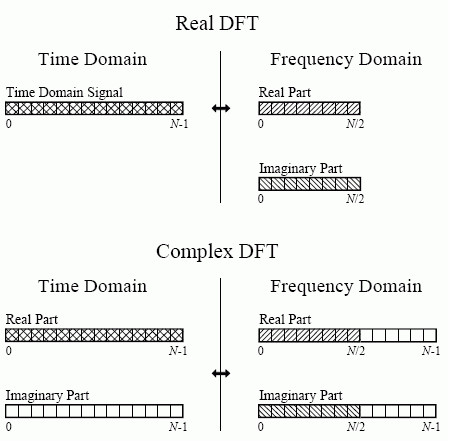
\includegraphics[width=\textwidth, keepaspectratio=true]{F_12_1}
\caption{Comparing the \textbf{real} and \textbf{complex} DFTs.
The real DFT takes an \textbf{N point} time domain signal and creates \textbf{two N/2-1} point frequency domain %signals. The \textbf{complex DFT} takes two N point time domain signals and creates two N point frequency domain signals. The crosshatched regions shows
the values common to the two transforms.}
\end{figure}


The \textbf{FFT} is based on the \textbf{complex DFT}.
Since the FFT is an algorithm for calculating the complex DFT. \autoref{fig:F_12_1} compares how the real DFT and the complex DFT store data.\\

The \textbf{real DFT} transforms an \textbf{N point} time domain signal into
\textbf{two N/2} + 1 point frequency domain signals. The time domain
signal is called just that: the \textbf{time domain signal}. The two signals in the
\textbf{frequency domain} are called the \textbf{real part} and the \textbf{imaginary part},
holding the \textbf{amplitudes of the cosine waves and sine waves}, respectively.
In comparison, the \textbf{complex DFT transforms} \textbf{two N point} time domain signals
into \textbf{two N point} frequency domain signals. The two time domain signals are
called the \textbf{real part} and the \textbf{imaginary part}, just as are the frequency domain
signals.
\\Suppose you have \textbf{an N point} signal, and need to calculate the \textbf{real DFT} by
means of the \textbf{Complex DFT} (such as by using the FFT algorithm).\\
\textbf{First}, move the \textbf{N point} signal into the \textbf{real part} of the \textbf{complex DFT's} time domain.\\
\textbf{Second}, set all of the samples in the \textbf{imaginary} part to \textbf{zero}.\\
\textbf{Third}, calculation of the \textbf{complex DFT} results in a \textbf{real} and an \textbf{imaginary} signal in the frequency domain, each composed of \textbf{N} points.
Samples 0 through N/2 of these signals correspond to the \textbf{real DFT's} spectrum.\\
The DFT's frequency domain is \textbf{periodic} when the negative frequencies are included (see Fig. 10-9).
The complex DFT's frequency spectrum includes the negative frequencies in the 0
to 1.0 arrangement. In other words, one full period stretches from sample 0 to
sample N-1 , corresponding with 0 to 1.0 times the sampling rate. The positive
frequencies sit between sample 0 and N/2 , corresponding with 0 to 0.5. The
other samples, between N/2 + 1 and N-1 , contain the negative frequency
values (which are usually ignored). \cite{smith1997dspbook}

\subsection{Continuous Fourier Transform}

%------------------------------------------------

\section{Results}

\begin{table}[H]
\caption{Example table}
\centering
\begin{tabular}{llr}
\toprule
\multicolumn{2}{c}{Name} \\
\cmidrule(r){1-2}
First name & Last Name & Grade \\
\midrule
%John & Doe & $7.5$ \\
%Richard & Miles & $2$ \\
\bottomrule
\end{tabular}
\end{table}

%\lipsum[5] % Dummy text

\begin{equation}
\label{eq:emc}
e = mc^2
\end{equation}

%\lipsum[6] % Dummy text

%------------------------------------------------

\section{Discussion}


%----------------------------------------------------------------------------------------
%	REFERENCE LIST
%----------------------------------------------------------------------------------------
\clearpage
%\markboth{Bibliografia}{Bibliografia}
%\printbibliography
%\bibliography{abbr_long,pubext}
\bibliographystyle{ieeetr}
\bibliography{thomastsai.bib}

%\begin{thebibliography}{99} % Bibliography - this is intentionally simple in this template

%\bibitem[Figueredo and Wolf, 2009]{Figueredo:2009dg}
%Figueredo, A.~J. and Wolf, P. S.~A. (2009).
%\newblock Assortative pairing and life history strategy - a cross-cultural
%  study.
%\newblock {\em Human Nature}, 20:317--330.

%\end{thebibliography}

%----------------------------------------------------------------------------------------

%\end{multicols}

\end{document}
